\documentclass[11pt]{article}
\usepackage{algpseudocode}
\usepackage{amsmath, amssymb, amsfonts}
\usepackage[english]{babel}
\usepackage{inputenc}
\usepackage{multicol}
\usepackage{flushend}
\usepackage{fullpage}
\usepackage{epsfig}
\usepackage{caption}
\captionsetup[table]{labelsep=period}
\usepackage{multirow}
\usepackage{mathtools}
\usepackage{xcolor}
\DeclarePairedDelimiter{\ceil}{\lceil}{\rceil}

\topmargin=-0.2in
\textheight=9.5in

\pagestyle{empty}

\begin{document}

\centerline{CSCE 614 (Fall 2020) \hfill Uwacu and Elsheimy}
\medskip
\centerline{\bf Computer Architecture}
\medskip

\centerline{\bf  Project report: }

\bigskip

\centerline{\bf Exploring Predictive Replacement Policies for Instruction Cache and Branch Target Buffer}

\bigskip

\centerline{\bf Diane Uwacu and Fatmaelzahraa Elsheimy}

\bigskip

\begin{abstract}
Many of the new-era processors support fetching instructions with instruction cache and branch target buffer. I-Cache and branch target buffer have limited capacities and
therefore, different types of replacement policies are being explored to reduce the misses in I-cache and BTB. In this project, we implement a new policy Global History Reuse 
Prediction (GHRP), a replacement policy that uses the history of previous instructions and behaviour predict and evict dead blocks. GHRP is implemented in the main paper using
Championship Branch Prediction simulator, but we try to implement it using Zsim to test the easiness of implementing the new policy in different simulators. GHRP’s performance
is compared against the famous policy LRU (Least recently used) and SRRIP(static re-reference interval prediction). Using Championship simulator, GHRP reduces the I-cache misses (MPKI) by 18% 
over LRU policy on a 662 industrial workloads. In Zsim, LRU data is collected over PARSEC benchmark and the results are speculated from the Championship results.
\end{abstract}

\section{Introduction} 
\label{sec:introduction}

Current processors need efficient instruction fetch for high performance. There are two main structures that the processor rely on for efficient fetching: I-cache and branch
target buffer. The instruction cache (I-cache) keeps record of recently used instructions, and the branch target buffer (BTB) caches targets of previously taken branches.
Therefore, the I-cache helps in improving instruction throughput and latency. Branch target buffer improves latency because of branch target-recomputation. This 
paper \cite{samira-ISCA18} explores efficient replacement policies at the I-cache and BTB levels. Samira et-al introduces a new idea for policy replacement called Graph History
Reuse Prediction. This algorithm is based on the history of past instruction addresses and behaviour in order to predict dead blocks in an efficient way. Predicting dead blocks
is very important as they free up space for other blocks that might be used in the future. A block is said to be dead if it is not going to be used before eviction. A block is 
said to be live if it is going to be used before eviction. Samira et-al have done a survey on the current implemented policies such as LRU, SSRIP..etc and tried to find a 
better policy. Most of the work on _cache optimization focused on instruction prefetching and block reordering. Many of these solutions didn’t lead to good  outcome as it 
resulted in large overhead or high MPKI. Similarly, most of the work on BTB optimization focused on the design structure or using different replacement policy. Again, the 
results weren’t that satisfactory. 
Samira et-al first, tried to apply PC-based predictor that uses set-sampling for Cache behavior generalization, however, when being applied on I-cache and BTB, they haven’t 
seen prominent results and hence, this idea was discarded. On the other side,  based on the survey done over all current replacement policies, they noted that that sequences of
recently accessed instructions correlate with the likelihood of block reuse. Their proposes policy results in a prominent improvement in cache efficiency and overall 
performance. They evaluated seven recent replacement policies and compared them based on average MPKI values. While, Samira et al applied their policy on Championship 
simulator. We have tried applying it on Zsim to test the ease of implementation of the policies in different simulators and compare the results using different benchmark; 
PARSEC.


\section{Background}
\label{sec:background}

Most other publications has only considered enhancing prefetching methods or software-based approaches. We are focusing our 
effort on improving replacement policies in I-cache and BTB based on dead-block prediction. When looking at recent work studying 
the effect of replacement policy, not many were found or mostly gave poor results \cite{ship-micro-2011, ISCA-2006} . Most of them focused on different approaches 
such as recent static prediction \cite{rrip-2010} and using a hashed value for indexing branch predictors table \cite{acm-2005}. Other works that studied dead-block 
prediction mainly focused on using it in power reduction \cite{IATAC-2005}, cache optimization \cite{ieeeCAT-2000} or bypassing \cite{johnson-1999}. Hence, our efforts will be focus on studying the use of dead block prediction
in the I-cache and BTB. Different algorithms will be tested to be able to adapt the dead block information to BTB and I-cache replacement using open-source simulator.  

According to authors, not much work has been done to evaluate replacement policies on the I-cache and BTB level. Except for the work in \cite{smith-1985} that was done in the 80s
with simpler policies like FIFO, and the work by Perleberg et al \cite{perleberg-1993} from the 90s, this is the first recent work to look at this problem from this angle.

Authors discuss how different prediction replacement policies affect and are affected by the I-cache and BTB. In particulat, they showed how a sampling-based
prediction policy that works well for PC-based dead block prediction, does not work as well in this area, due to the fact that a given PC only accesses one set at a time.
In addition to the sampling-based method, authors compare their work againt the least recently-used (LRU) policy, the random policy, and the static re-reference predictor (SRRIP).


\section{Work Description}
\label{sec:Work Description}
The GHRP method uses past history to predict dead-blocks in the cache.
It indexes a table of counters with a signature generated from features correlated with reuse behavior using the global path history
of instruction addresses.
The global history is updated by shifting three lowest-order bits of the PC, and the signature is found by exclusive-ORing the history with the PC.
GHRP uses three hash tables that provide a prediction via majority vote.
With a 64kB I-cache with a 64B block size, we created three prediction tables with 4096 entires and a two-bit counter per entry.
\par

Our plan was to implement the Global History Replacement Policy (GHRP) method as described in the paper, and assess its performance by comparing it to the LRU method.
The method was implemented using a simulator that we were not familiar with, so we decided to implement the logic in the zsim simulator instead.
Algorithm \ref{alg1} describes our implementation. We split Algorithm 1 of \cite{samira-ISCA18} into three procedures that are required to use the Cache classes in zsim.\par

The update() function is used in zsim to update the prediction tables after a hit. In our implementation, we called updatePredTables() without flagging that the block is dead, as detailed in Algorithm 1 of \cite{samira-ISCA18}. 
The replaced() function is used in zsim to replace In our implementation, we called updatePredTables(), and this time we that the block is dead, as detailed in Algorithm 1 of \cite{samira-ISCA18}.
The rank() function is used in zsim to rank replacement cadidates. In our implementation, we used the MajorityVote() function detailed in Algorithm 1 of \cite{samira-ISCA18} that is used on the hashed indices from the three prediction tables to find a block to update or replace depending on how the flag is set.\par

To fall back to a LRU replacement when there is no block picked by the GHRP method, we added an implementation of LRU replacement in our implementation.
We did not get a chance to adapt the method for BTB replacement due to time restrictions.
%%% Algorithm 1 Pseudocode
%\begin{algorithm}[h]
	%\label{alg:alg1}
	\begin{algorithmic}[1]
	%\caption{GHRP}
		\renewcommand{\algorithmicrequire}{\textbf{Input: PC}}
		%\REQUIRE int PC
		\Procedure{update}{id, req}
		\State{${\tt UpdatePredTable}(id, req)$}
		\EndProcedure
		\Procedure{replaced}{id, req}
		\State{${\tt UpdatePredTable}(id, req)$}
		\EndProcedure
		\Procedure{rank}{id, req}
		\State{${\tt UpdatePredTable}(id, req)$}
		\EndProcedure
	\end{algorithmic}
%\end{algorithm}

\section{Evaluation}
\label{sec:Evaluation}

\subsection{Experimental Setup - Diane}
We opted to implement the method in zsim since we were more familiar with the simulator, and we thought that the paper provided enough information to implement the method.
However, we realized a bit late that this was not the case. Apart from the difference in data structures, certain components that are explicitely updated in the method were assumed to be computed by the Cache class in zsim, and thus outside of the scope of the replacement policy code.\par
We were able to implement the code, but we were unable to link it to the Cache class properly to be able to run experiments as it was difficult to adapt it to the current zsim architecture. 
In this section, we will discuss the performance of GHRP compared to SRRIP and LRU polices over PARSEC benchmark. These are speculations done by comparing our LRU results to the paper's results.

\subsection{Experimental Results and Discussion}
In order to compare the efficiency of the GHRP policy, it was implemented on two different simulators; Champ and Zsim. In the paper, Samira et al implement the policy using
Champ and comparing it with other policies such as LRU, and SRRIP on industrial benchmarks. In our project, we tried implementing on Zsim and comparing the results against 
SRRIP and LRU on PARSEC benchmark. Unfortunately, due to Zsim architecture and the way the policies are implemented. It was difficult to implement the GHRP policy in the 
current Zsim architecture. We collected data from Samira et al as well as collected data from the  LRU AND SRRIP on PARSEC and we speculated the results by GHRP. In figure 1,
It shows the results of the implementation of different policies on an 8-way 64KB I-cache with 64B blocks using Champ simulator. Figure 1 shows the results of these policies in
relative to the MPKI of the LRU. On average of the 662 workloads, GHRP has a lower MPKI average of 0.86 compared with 1.02 for SRRIP and 1.10 for SDBP. By percentage, GHRP 
improves the average MPKI by 18% over LRU and 12% over SRRIP. In the 2nd figure, Samira et al explored other configuration of the I-cache. In figure 2,  it shows various 
combinations of 8KB,  16KB, 32KB and 64KB caches with 64B blocks with 4-way or 8-way associativity. It can be clearly seen how GHRP outperformed all other policies. LRU has
performed the worst results by average of 10% less than other policies. GHRP has reduced the average of the MPKI by 14% compared to the LRU results.
Using Zsim, GHRP is compared against LRU and SRRIP on PARSEC benchmark. The MPKI value is calculated using the following equations:  
total misses = mGETS + mGETXIM + mGETXSM

MPKI = (total misses/total instruction)*1000
Where mGETS are misses of the GETS , mGETXIM are the
misses of GETXI => M, and mGETXSM are the misses
of the GETXS => M .

\begin{figure}[h]
	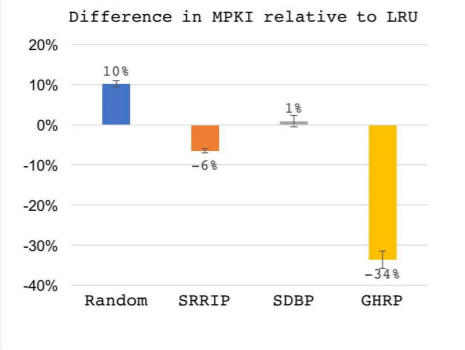
\includegraphics[width=1\textwidth]{report1.PNG}
	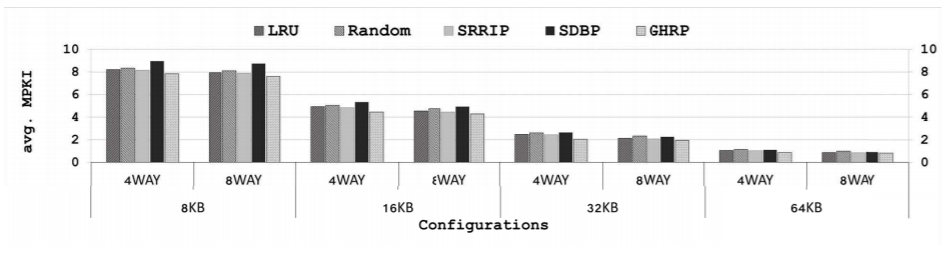
\includegraphics[width=1\textwidth]{reportresult.PNG}
\end{figure}

Figures 3 and 4 display the results of the policies over the PARSEC benchmarks. The value of the MPKI for each policy was calculated using the above mentioned equations and
recorded in figure 3. It can be clearly shown the LRU has done the worst compared to all of them. SRRIP has done better than LRU by average of 10%. According to Samira’s 
results, the GHRP is expected to outperform both LRU and SRRIP by average of 8% when compared with the previous results from figures 1 and 2. 
The analysis behind such results is due to the algorithm and the core idea of GHRP. GHRP targets the removal of dead blocks/BTB entries by using the history of past 
instructions addresses and behavior. LRU just uses information based on the last recently used block, which isn’t really efficient to detect dead blocks especially when it does
not think that the most recent entry will be re-referenced in
the near-immediate future. In results, LRU is inefficient especially with applications that its referenced mainly in the distant future. LRU replaces the blocks very 
frequently. 
 SSRIP uses lower hardware overhead and deals better with applications with larger working sets and applications with references in the distant future than LRU. SSRIP has two 
kinds of priorities: Hit priority and Frequency priority. For this project, the Hit priority one was implemented. Therefore, it can be deduced that many of the PARSEC 
benchmarks have blocks that are referenced in the distant future and that’s why SRRIP outperformed LRU. For GHRP, it can predict dead blocks in application with larger worker 
sets and references in the distant future better than both SRRIP and LRU. SRRIP uses 2 bits per cache block to store 2^2 prediction values (RRVP)for scan resistant, which means
a block has 4 chances before being evicted. GHRP doesn’t face this problem as it bases its prediction on indexing a table of counters with a signature generated by correlated 
it to data from previous history. The final prediction is passed by majority vote which further improves the assurance of the prediction. Hence, a block has a better chance to 
stay in cache before being evicted. Overall, GHRP better predict dead blocks than SRRIP and LRU. 

\begin{figure}[h]
	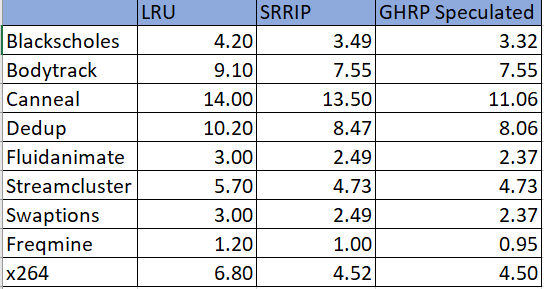
\includegraphics[width=1\textwidth]{MPKI1.PNG}
	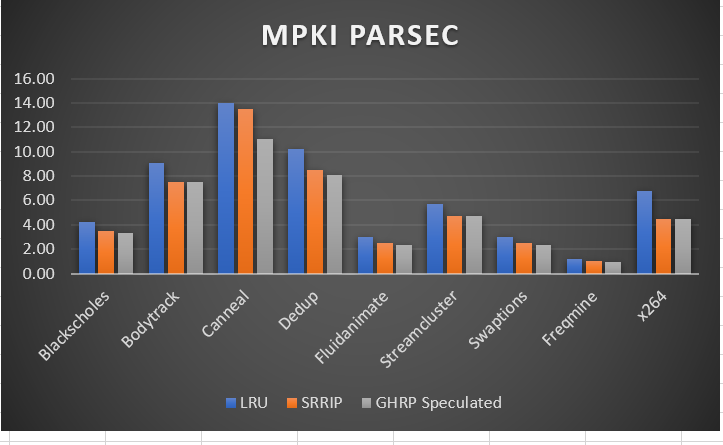
\includegraphics[width=1\textwidth]{MPKI2.PNG}
\end{figure}

\section{Conclusion and Future Work}
We implemented the global history replacement policy in zsim and made enough progress to show that it is realizable in a different simulator than originally presented. However, due to zsim setup and the time constraint, it wasn't very easy to implement GHRP in a way that's adaptable to the current architecture. However, we still implemenetd the algorithms fully in zsim as shown in the pseudocode. 
Based on the results in the paper and the extrapolation done, it is clearly shown that GHRP outperforms all the other policies. In this project, we compared it against LRU and SRRIP, and GHRP shown a better performance by reduing the MPKI by average of 10%.
For future work, it would be great to try implementting the policy on other tools other than zsim and Championship and tests its performance on other benchmarks as well. 

{%\scriptsize
	\bibliographystyle{abbrv}
	\bibliography{references}
	}

\end{document}



